% ==============================================================================
% Lista de Exercicios - Programacao Linear Inteira (CEMMA)
% Prof. Franklin Angelo Krukoski - Junho/2026
% ==============================================================================
\documentclass[11pt, a4paper]{article}

\usepackage[utf8]{inputenc}
\usepackage[T1]{fontenc}
\usepackage[brazil]{babel}
\usepackage[top=2.5cm, bottom=2.5cm, left=2.5cm, right=2.5cm]{geometry}
\usepackage{times}
\usepackage{microtype}

\usepackage{amsmath, amssymb}
\usepackage{booktabs}
\usepackage{longtable}
\usepackage{graphicx}
\usepackage{float}
\usepackage{caption}
\captionsetup{font=small, labelfont=bf}
\usepackage{xcolor}
\usepackage{listings}
\usepackage{enumitem}
\usepackage[hidelinks]{hyperref}
\usepackage{fancyhdr}

\graphicspath{{../figs/}}

\pagestyle{plain}

% --- estilo de codigo Python ---
\definecolor{codegreen}{rgb}{0.0,0.5,0.0}
\definecolor{codegray}{rgb}{0.5,0.5,0.5}
\definecolor{codeblue}{rgb}{0.1,0.1,0.6}
\definecolor{backcolour}{rgb}{0.96,0.96,0.94}
\lstdefinestyle{py}{
  backgroundcolor=\color{backcolour}, commentstyle=\color{codegreen},
  keywordstyle=\color{codeblue}\bfseries, stringstyle=\color{codegreen},
  basicstyle=\ttfamily\footnotesize, breaklines=true, captionpos=b,
  keepspaces=true, numbers=left, numbersep=5pt, numberstyle=\tiny\color{codegray},
  showstringspaces=false, frame=single, language=Python, tabsize=2}
\lstset{style=py}

\newcommand{\R}{\mathbb{R}}
\newcommand{\Z}{\mathbb{Z}}

\begin{document}

% --------------------------- CAPA ---------------------------
\begin{titlepage}
\centering
\vspace*{4cm}
{\Large\textbf{Resolu\c{c}\~ao da Lista de Exerc\'icios}}\\[1em]
{\large Programa\c{c}\~ao Linear Inteira}\\[3cm]
{\normalsize Ettore Gabriel Emilio Reis Braga}\\[0.6em]
{\normalsize Especializa\c{c}\~ao em M\'etodos Matem\'aticos Aplicados (CEMMA)}\\[0.3em]
{\normalsize Prof.\ Franklin Angelo Krukoski}\\[3cm]
{\normalsize Junho de 2026}
\end{titlepage}

%\tableofcontents
\newpage

% ============================================================================
\section{Parte 1: Constru\c{c}\~ao da \'Arvore Branch-and-Bound}
% ============================================================================
Foi utilizado o solver PuLP em Python para os problemas.
\textbf{Estrat\'egia de busca adotada: busca em profundidade} (\emph{depth-first
search}). A cada n\'o resolve-se a relaxa\c{c}\~ao linear (vari\'aveis cont\'inuas)
com o CBC. \textbf{Regra de ramifica\c{c}\~ao:} escolhe-se a vari\'avel inteira de
\emph{menor \'indice} cujo valor na relaxa\c{c}\~ao seja fracion\'ario. Cada \emph{passo}
corresponde \`a resolu\c{c}\~ao da relaxa\c{c}\~ao de um n\'o.

\medskip
\noindent\textbf{Crit\'erios de poda:} (i) \emph{inviabilidade}: a relaxa\c{c}\~ao
do n\'o n\~ao tem solu\c{c}\~ao; (ii) \emph{integralidade}: a solu\c{c}\~ao da
relaxa\c{c}\~ao j\'a \'e inteira (candidata a incumbente); (iii) \emph{limitante}
(\emph{bound}): o valor da relaxa\c{c}\~ao n\~ao supera o incumbente corrente.

\medskip
\noindent Nas figuras: \textcolor{blue}{\textbf{azul}} = n\'o fracion\'ario
(ramificado), \textcolor{green!60!black}{\textbf{verde}} = solu\c{c}\~ao inteira,
\textcolor{orange}{\textbf{laranja}} = podado por limitante,
\textcolor{red}{\textbf{vermelho}} = inviavel. O r\'otulo $p_k$ indica o passo.

\medskip
\noindent O trecho central do motor de B\&B (resolu\c{c}\~ao da relaxa\c{c}\~ao de
cada n\'o) \'e:
\begin{lstlisting}
import pulp
def solve_relaxation(prob, bounds):
    m = pulp.LpProblem("relax", prob["sense"])          # Maximize/Minimize
    x = {n: pulp.LpVariable(n, *bounds.get(n,(0,None)),  # limites do no
                            cat="Continuous") for n in prob["vars"]}
    m += pulp.lpSum(prob["obj"].get(n,0)*x[n] for n in prob["vars"])
    for coef, sign, rhs in prob["constraints"]:
        e = pulp.lpSum(coef.get(n,0)*x[n] for n in prob["vars"])
        m += (e <= rhs) if sign=="<=" else (e >= rhs) if sign==">=" else (e == rhs)
    m.solve(pulp.PULP_CBC_CMD(msg=0))
    return pulp.value(m.objective), {n: x[n].value() for n in prob["vars"]}
\end{lstlisting}

% ---------- Exercicio 1 ----------
\subsection{Exerc\'icio 1}
\[
\max z = x_1+5x_2+9x_3+5x_4 \quad\text{s.a.}\quad
\begin{cases}
x_1+3x_2+9x_3+6x_4 \le 16\\
6x_1+6x_2+7x_4 \le 19\\
7x_1+8x_2+18x_3+3x_4 \le 44\\
x_1,x_2,x_3,x_4 \ge 0\ \text{e inteiras.}
\end{cases}
\]
A relaxa\c{c}\~ao na raiz fornece $z=22{,}33$ (fracion\'aria). A busca em
profundidade explora 13 n\'os at\'e a \'arvore completa. A sequ\^encia de passos
est\'a na tabela; a \'arvore na Figura~\ref{fig:p1ex1}.
\begin{footnotesize}
\begin{longtable}{c c l c l c p{4.2cm}}
\toprule
Passo & N\'o & Ramo & $z_{LP}$ & Solu\c{c}\~ao da relaxa\c{c}\~ao & Status & Observa\c{c}\~ao \\
\midrule
\endhead
1 & N0 & raiz (LP) & 22.333 & x1=0, x2=3.17, x3=0.72, x4=0 & fracion. & Ramifica em x2 = 3.167 \\
2 & N1 & x2 $\leq$ 3 & 22.000 & x1=0, x2=3, x3=0.78, x4=0 & fracion. & Ramifica em x3 = 0.778 \\
3 & N3 & x3 $\leq$ 0 & 15.714 & x1=0, x2=3, x3=0, x4=0.14 & fracion. & Ramifica em x4 = 0.143 \\
4 & N5 & x4 $\leq$ 0 & 15.167 & x1=0.17, x2=3, x3=0, x4=0 & fracion. & Ramifica em x1 = 0.167 \\
5 & N7 & x1 $\leq$ 0 & 15.000 & x1=0, x2=3, x3=0, x4=0 & inteira & Nova solucao incumbente (inteira) \\
6 & N8 & x1 $\geq$ 1 & 11.833 & x1=1, x2=2.17, x3=0, x4=0 & podado & Poda por limitante (z=11.833 nao supera incumbente 15.000) \\
7 & N6 & x4 $\geq$ 1 & 15.000 & x1=0, x2=2, x3=0, x4=1 & podado & Poda por limitante (z=15.000 nao supera incumbente 15.000) \\
8 & N4 & x3 $\geq$ 1 & 20.667 & x1=0, x2=2.33, x3=1, x4=0 & fracion. & Ramifica em x2 = 2.333 \\
9 & N9 & x2 $\leq$ 2 & 20.000 & x1=0, x2=2, x3=1.11, x4=0 & fracion. & Ramifica em x3 = 1.111 \\
10 & N11 & x3 $\leq$ 1 & 20.000 & x1=1, x2=2, x3=1, x4=0 & inteira & Nova solucao incumbente (inteira) \\
11 & N12 & x3 $\geq$ 2 & -- & -- & inviavel & Poda por inviabilidade \\
12 & N10 & x2 $\geq$ 3 & -- & -- & inviavel & Poda por inviabilidade \\
13 & N2 & x2 $\geq$ 4 & -- & -- & inviavel & Poda por inviabilidade \\
\bottomrule
\end{longtable}
\end{footnotesize}

\begin{figure}[H]\centering
  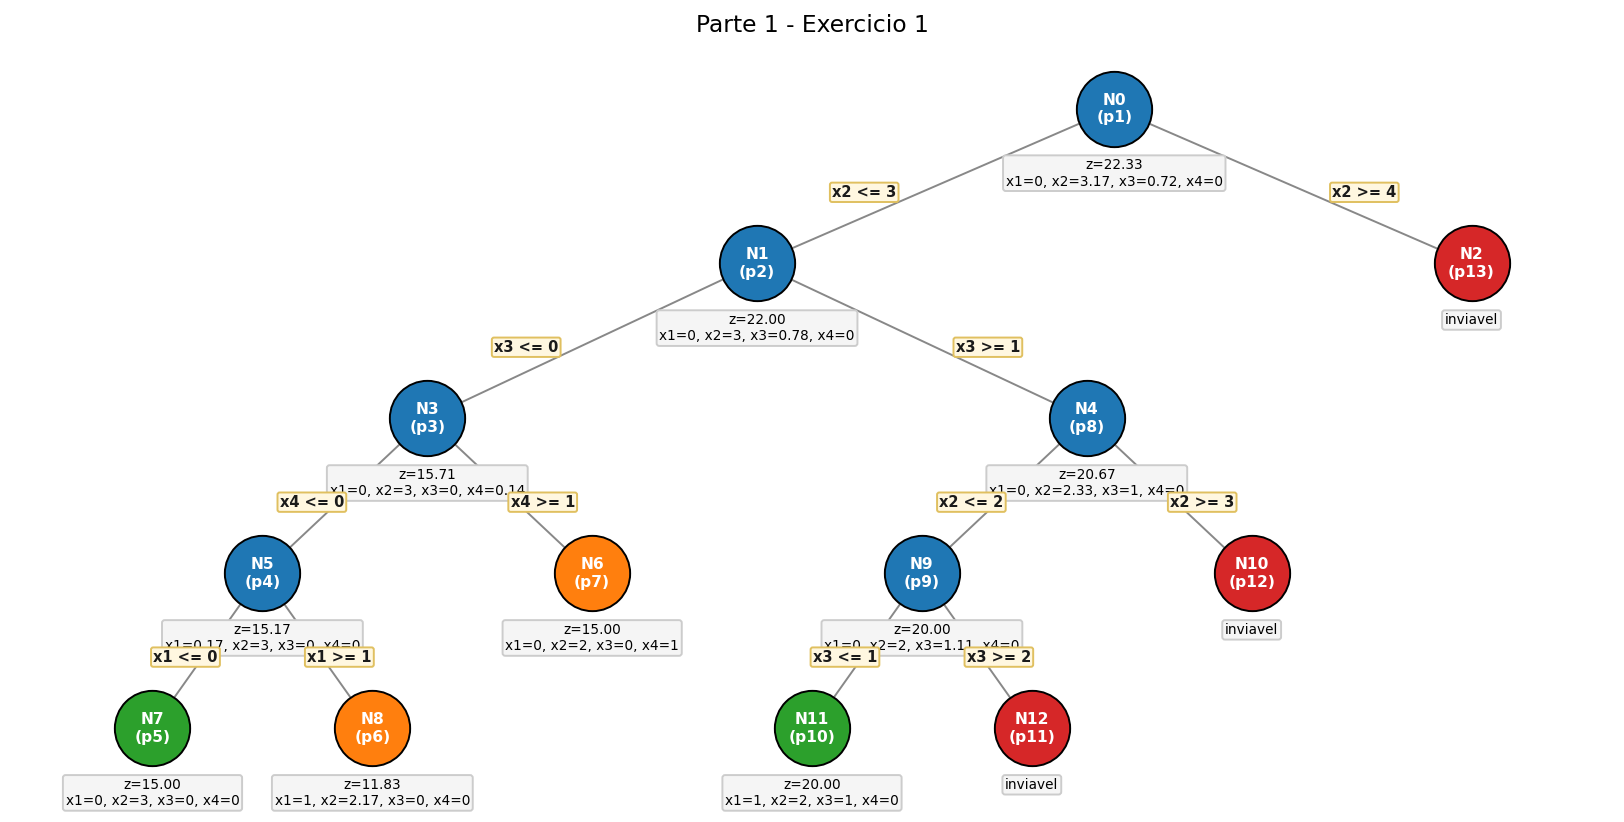
\includegraphics[width=\linewidth]{p1_ex1_tree.png}
  \caption{\'Arvore B\&B completa, Parte 1, Exerc\'icio 1.}\label{fig:p1ex1}
\end{figure}
\noindent\textbf{Solu\c{c}\~ao \'otima:} $z^{*}=20$ em $(x_1,x_2,x_3,x_4)=(1,2,1,0)$
(n\'o N11).

% ---------- Exercicio 2 ----------
\subsection{Exerc\'icio 2}
\[
\max z = 7x_1+9x_2+x_3+6x_4 \quad\text{s.a.}\quad
\begin{cases}
8x_1+2x_2+4x_3+2x_4 \le 16\\
4x_1+8x_2+2x_3 \le 20\\
7x_1+6x_3+2x_4 \le 11\\
x_1,x_2,x_4 \ge 0\ \text{inteiras};\ x_3 \ge 0.
\end{cases}
\]
Aqui $x_3$ \'e cont\'inua, portanto a ramifica\c{c}\~ao incide apenas sobre
$x_1,x_2,x_4$. A \'arvore completa tem 7 n\'os.
\begin{footnotesize}
\begin{longtable}{c c l c l c p{4.2cm}}
\toprule
Passo & N\'o & Ramo & $z_{LP}$ & Solu\c{c}\~ao da relaxa\c{c}\~ao & Status & Observa\c{c}\~ao \\
\midrule
\endhead
1 & N0 & raiz (LP) & 55.500 & x1=0, x2=2.5, x3=0, x4=5.5 & fracion. & Ramifica em x2 = 2.500 \\
2 & N1 & x2 $\leq$ 2 & 51.000 & x1=0, x2=2, x3=0, x4=5.5 & fracion. & Ramifica em x4 = 5.500 \\
3 & N3 & x4 $\leq$ 5 & 49.000 & x1=0.14, x2=2, x3=0, x4=5 & fracion. & Ramifica em x1 = 0.143 \\
4 & N5 & x1 $\leq$ 0 & 48.167 & x1=0, x2=2, x3=0.17, x4=5 & inteira & Nova solucao incumbente (inteira) \\
5 & N6 & x1 $\geq$ 1 & 37.000 & x1=1, x2=2, x3=0, x4=2 & podado & Poda por limitante (z=37.000 nao supera incumbente 48.167) \\
6 & N4 & x4 $\geq$ 6 & -- & -- & inviavel & Poda por inviabilidade \\
7 & N2 & x2 $\geq$ 3 & -- & -- & inviavel & Poda por inviabilidade \\
\bottomrule
\end{longtable}
\end{footnotesize}

\begin{figure}[H]\centering
  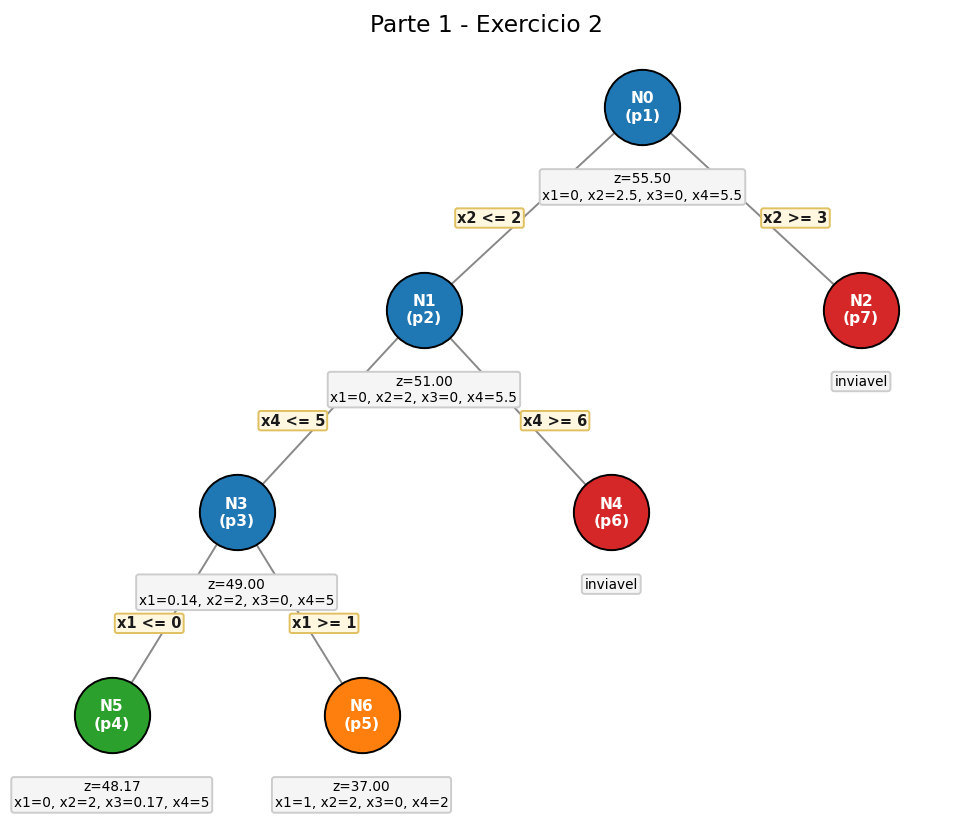
\includegraphics[width=0.92\linewidth]{p1_ex2_tree.png}
  \caption{\'Arvore B\&B completa, Parte 1, Exerc\'icio 2.}\label{fig:p1ex2}
\end{figure}
\noindent\textbf{Solu\c{c}\~ao \'otima:} $z^{*}=48{,}1\overline{6}=\tfrac{289}{6}$ em
$(x_1,x_2,x_3,x_4)=(0,\,2,\,\tfrac16,\,5)$.

% ---------- Exercicio 3 ----------
\subsection{Exerc\'icio 3}
\[
\min z = 3x_1+4x_2+3x_3 \quad\text{s.a.}\quad
\begin{cases}
3x_1+2x_2+2x_3 \ge 13\\
2x_1+5x_2+3x_3 \ge 15\\
2x_1+x_2+2x_3 \ge 9\\
x_2,x_3 \ge 0\ \text{inteiras};\ x_1 \ge 0.
\end{cases}
\]
$x_1$ \'e cont\'inua; ramifica-se sobre $x_2,x_3$. A \'arvore completa tem 9 n\'os.
\begin{footnotesize}
\begin{longtable}{c c l c l c p{4.2cm}}
\toprule
Passo & N\'o & Ramo & $z_{LP}$ & Solu\c{c}\~ao da relaxa\c{c}\~ao & Status & Observa\c{c}\~ao \\
\midrule
\endhead
1 & N0 & raiz (LP) & 16.556 & x1=2.78, x2=1.22, x3=1.11 & fracion. & Ramifica em x2 = 1.222 \\
2 & N1 & x2 $\leq$ 1 & 16.600 & x1=2.6, x2=1, x3=1.6 & fracion. & Ramifica em x3 = 1.600 \\
3 & N3 & x3 $\leq$ 1 & 17.500 & x1=3.5, x2=1, x3=1 & inteira & Nova solucao incumbente (inteira) \\
4 & N4 & x3 $\geq$ 2 & 16.636 & x1=2.45, x2=0.82, x3=2 & fracion. & Ramifica em x2 = 0.818 \\
5 & N5 & x2 $\leq$ 0 & 16.800 & x1=1.8, x2=0, x3=3.8 & fracion. & Ramifica em x3 = 3.800 \\
6 & N7 & x3 $\leq$ 3 & 18.000 & x1=3, x2=0, x3=3 & podado & Poda por limitante (z=18.000 nao supera incumbente 17.500) \\
7 & N8 & x3 $\geq$ 4 & 17.000 & x1=1.67, x2=0, x3=4 & inteira & Nova solucao incumbente (inteira) \\
8 & N6 & x2 $\geq$ 1 & 17.000 & x1=2.33, x2=1, x3=2 & podado & Poda por limitante (z=17.000 nao supera incumbente 17.000) \\
9 & N2 & x2 $\geq$ 2 & 18.500 & x1=3.5, x2=2, x3=0 & podado & Poda por limitante (z=18.500 nao supera incumbente 17.000) \\
\bottomrule
\end{longtable}
\end{footnotesize}

\begin{figure}[H]\centering
  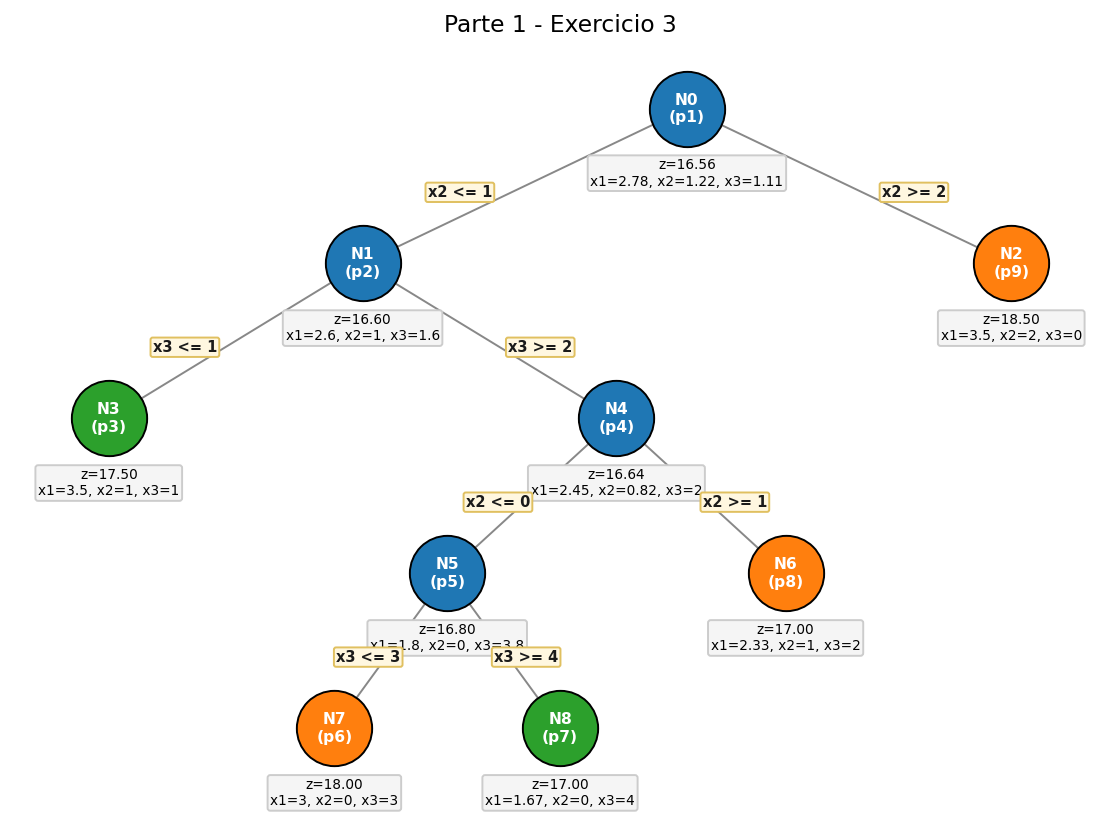
\includegraphics[width=0.92\linewidth]{p1_ex3_tree.png}
  \caption{\'Arvore B\&B completa, Parte 1, Exerc\'icio 3.}\label{fig:p1ex3}
\end{figure}
\noindent\textbf{Solu\c{c}\~ao \'otima:} $z^{*}=17$ em
$(x_1,x_2,x_3)=(\tfrac53,\,0,\,4)$.

% ---------- Exercicio 4 ----------
% \subsection{Exerc\'icio 4}
% \[
% \min z = 2x_1+3x_2+5x_3 \quad\text{s.a.}\quad
% \begin{cases}
% x_1+2x_2+3x_3 \ge 7\\
% 3x_1+2x_2+3x_3 \ge 11\\
% x_1,x_3 \ge 0\ \text{inteiras};\ x_2 \ge 0.
% \end{cases}
% \]
% \begin{footnotesize}
\begin{longtable}{c c l c l c p{4.2cm}}
\toprule
Passo & N\'o & Ramo & $z_{LP}$ & Solu\c{c}\~ao da relaxa\c{c}\~ao & Status & Observa\c{c}\~ao \\
\midrule
\endhead
1 & N0 & raiz (LP) & 11.500 & x1=2, x2=2.5, x3=0 & inteira & Nova solucao incumbente (inteira) \\
\bottomrule
\end{longtable}
\end{footnotesize}

% \noindent Neste caso a relaxa\c{c}\~ao na raiz j\'a fornece valores inteiros para
% as vari\'aveis exigidas inteiras ($x_1=2$, $x_3=0$, com $x_2=2{,}5$ cont\'inua).
% Logo a \'arvore se encerra na raiz, \emph{sem necessidade de ramifica\c{c}\~ao}.
% \textbf{Solu\c{c}\~ao \'otima:} $z^{*}=11{,}5$ em $(x_1,x_2,x_3)=(2,\,2{,}5,\,0)$.

\newpage
% ============================================================================
\section{Parte 2: Formula\c{c}\~ao de Problemas de PLI}
% ============================================================================
Apresentam-se apenas os modelos matem\'aticos (vari\'aveis de decis\~ao, fun\c{c}\~ao
objetivo e restri\c{c}\~oes), conforme solicitado.

% ---------- Ex1 ----------
\subsection{Exerc\'icio 1: Carregamento do avi\~ao cargueiro}
\textbf{Vari\'aveis de decis\~ao.} Para os cont\^eineres dos tipos $i\in\{1,2,3\}$
e compartimentos $k\in\{F,C,T\}$ (frontal, central, cauda), seja
$n_{ik}\in\Z_{\ge 0}$ o n\'umero de cont\^eineres do tipo $i$ no compartimento $k$.
Para as cargas a granel $j\in\{4,5\}$ (apenas no por\~ao $G$), seja
$g_j \ge 0$ a quantidade (em toneladas) da carga $j$.

\noindent Pesos por contêiner $w_1{=}0{,}7,\,w_2{=}0{,}9,\,w_3{=}0{,}2$ (ton);
volumes $v_1{=}0{,}5,\,v_2{=}1,\,v_3{=}0{,}25$ (m$^3$). Densidades a granel
$1{,}2$ e $1{,}7$ ton/m$^3$. Lucros (\$/ton): $200,220,175,235,180$.

\textbf{Fun\c{c}\~ao objetivo} (maximizar o lucro, lucro = \$/ton $\times$ ton):
\[
\max\; z = \sum_{k}\big(200\,w_1 n_{1k}+220\,w_2 n_{2k}+175\,w_3 n_{3k}\big)
            + 235\,g_4 + 180\,g_5 .
\]
\textbf{Restri\c{c}\~oes de peso} (cap.\ em ton: $F{=}5,C{=}7,T{=}6,G{=}7$):
\[
\sum_i w_i n_{iF}\le 5,\quad \sum_i w_i n_{iC}\le 7,\quad
\sum_i w_i n_{iT}\le 6,\quad g_4+g_5 \le 7 .
\]
\textbf{Restri\c{c}\~oes de espa\c{c}o} (cap.\ em m$^3$: $F{=}35,C{=}55,T{=}30,G{=}30$):
\[
\sum_i v_i n_{iF}\le 35,\quad \sum_i v_i n_{iC}\le 55,\quad
\sum_i v_i n_{iT}\le 30,\quad \tfrac{g_4}{1{,}2}+\tfrac{g_5}{1{,}7}\le 30 .
\]
\textbf{Equil\'ibrio de voo} (peso proporcional \`a capacidade de cada compartimento):
\[
\frac{\sum_i w_i n_{iF}}{5}=\frac{\sum_i w_i n_{iC}}{7}
=\frac{\sum_i w_i n_{iT}}{6}=\frac{g_4+g_5}{7}.
\]
\[ n_{ik}\in\Z_{\ge0},\quad g_j\ge 0. \]

% ---------- Ex2 ----------
\subsection{Exerc\'icio 2: Combate ao inc\^endio florestal}
\textbf{Vari\'aveis:} $x_1,x_2,x_3\in\Z_{\ge0}$ = n\'umero de helic\'opteros AH-1,
avi\~oes-tanque e avi\~oes B67 mobilizados. A opera\c{c}\~ao dura $3$ horas.

\textbf{Objetivo} (minimizar custo $=3\,$h $\times$ custo/h):
\[ \min\; z = 3(2000x_1+4000x_2+10000x_3)=6000x_1+12000x_2+30000x_3 .\]
\textbf{Restri\c{c}\~oes:}
\[
\begin{aligned}
&3(15000x_1+40000x_2+85000x_3) \ge 3{.}000{.}000 &&\text{(\'area coberta)}\\
&2x_1 \le 10 &&\text{(pilotos de helic\'optero)}\\
&2x_2+2x_3 \le 14 &&\text{(pilotos de avi\~ao)}\\
&x_2+3x_3 \le 22 &&\text{(operadores)}\\
&x_1,x_2,x_3 \in \Z_{\ge0}.
\end{aligned}
\]

% ---------- Ex4 ----------
\subsection{Exerc\'icio 4: Redu\c{c}\~ao de peso do autom\'ovel}
\textbf{Vari\'aveis:} $x_j\in\{0,1\}$, $j=1,\dots,12$, igual a 1 se a altera\c{c}\~ao
$j$ for implementada. Sejam $r_j$ a redu\c{c}\~ao de peso (kg) e $c_j$ o custo (\$).
\[
\min\; z=\sum_{j=1}^{12} c_j x_j \qquad\text{s.a.}\qquad
\sum_{j=1}^{12} r_j x_j \ge 180,\qquad x_j\in\{0,1\}.
\]
com $r=(30,20,25,40,15,10,$ $60,80,40,30,50,35)$ e
$c=(130,110,120,150,80,80,$ $360,400,160,120,200,160)$ (em mil \$).

% ---------- Ex5 ----------
\subsection{Exerc\'icio 5: Localiza\c{c}\~ao de Centros de Distribui\c{c}\~ao}
\textbf{Vari\'aveis:} $y_i\in\{0,1\}$ = 1 se o CD do local $i$ \'e instalado
($i\in\{A,\dots,F\}$); $x_{ij}\ge0$ = quantidade (em 1.000 t) enviada do local $i$
ao distribuidor $j$ ($j=1,\dots,6$).

\noindent Par\^ametros: $f_i$ custo fixo, $v_i$ custo vari\'avel (\$/1.000t),
$\text{Cap}_i$ capacidade, $c_{ij}$ custo de transporte, $d_j$ demanda.
\[
\min\; z=\sum_i f_i y_i + \sum_i\sum_j (v_i+c_{ij})\,x_{ij}
\]
\[
\begin{aligned}
&\sum_i x_{ij} = d_j, && j=1,\dots,6 &&\text{(atender demanda)}\\
&\sum_j x_{ij} \le \text{Cap}_i\, y_i, && i\in\{A,\dots,F\} &&\text{(capacidade e abertura)}\\
&x_{ij}\ge 0,\quad y_i\in\{0,1\}.
\end{aligned}
\]
A restri\c{c}\~ao $\sum_j x_{ij}\le \text{Cap}_i y_i$ garante que s\'o se despacha de um
local \emph{aberto} ($y_i=1$).

% ---------- Ex6 ----------
% \subsection{Exerc\'icio 6: Plano de investimentos (Tupinamb\'a)}
% \textbf{Vari\'aveis:} $x_j\in\{0,1\}$, $j=1,\dots,10$, igual a 1 se o projeto $j$
% for selecionado. $\text{INV}_j$ = investimento e $\text{VP}_j$ = valor presente
% (em mil US\$).
% \[ \max\; z=\sum_{j=1}^{10}\text{VP}_j\,x_j \]
% \[
% \begin{aligned}
% &\sum_{j} \text{INV}_j\, x_j \le 400{.}000 &&\text{(or\c{c}amento US\$ 400 mi)}\\
% &\sum_{j} x_j \le 5 &&\text{(5 gerentes dispon\'iveis)}\\
% &x_2 \le x_1 &&\text{(2 complementar a 1)}\\
% &x_3 + x_4 \le 1 &&\text{(3 e 4 mutuamente exclusivos)}\\
% &x_5 \le x_4 &&\text{(5 complementar a 4)}\\
% &x_6 + x_7 \le 1 &&\text{(6 e 7 mutuamente exclusivos)}\\
% &x_8 + x_9 + x_{10} \le 1 &&\text{(8, 9 e 10 mutuamente exclusivos)}\\
% &x_8+x_9+x_{10} \le x_6+x_7 &&\text{(amplia\c{c}\~ao exige mat\'eria-prima 6 ou 7)}\\
% &x_8+x_9+x_{10} \le x_3+x_4 &&\text{(amplia\c{c}\~ao exige armazenagem 3 ou 4)}\\
% &x_j \in \{0,1\}.
% \end{aligned}
% \]

\newpage
% ============================================================================
\section{Parte 3: Transporte, Transbordo e Designa\c{c}\~ao}
% ============================================================================
Os problemas de transporte foram modelados como
$\min \sum_{ij} c_{ij}x_{ij}$ sujeito a
$\sum_j x_{ij}\le s_i$ (oferta) e $\sum_i x_{ij}= d_j$ (demanda), com
$x_{ij}\ge 0$, v\'alido pois em todos os casos a oferta total $\ge$ demanda
total. A fun\c{c}\~ao gen\'erica de resolu\c{c}\~ao (PuLP/CBC) utilizada foi:
\begin{lstlisting}
def solve_transport(cost, supply, demand):
    m = len(supply); n = len(demand)
    prob = pulp.LpProblem("transp", pulp.LpMinimize)
    x = [[pulp.LpVariable(f"x_{i}_{j}", lowBound=0) for j in range(n)]
          for i in range(m)]
    prob += pulp.lpSum(cost[i][j]*x[i][j] for i in range(m) for j in range(n))
    for i in range(m): prob += pulp.lpSum(x[i][j] for j in range(n)) <= supply[i]
    for j in range(n): prob += pulp.lpSum(x[i][j] for i in range(m)) == demand[j]
    prob.solve(pulp.PULP_CBC_CMD(msg=0))                # solver CBC
    return [[x[i][j].value() for j in range(n)] for i in range(m)], pulp.value(prob.objective)
\end{lstlisting}
O problema de designa\c{c}\~ao (Ex.\ 5) usa vari\'aveis bin\'arias $x_{ij}\in\{0,1\}$
com $\sum_j x_{ij}=1$ e $\sum_i x_{ij}=1$.

% ---------- Ex1 ----------
\subsection{Exerc\'icio 1: Transporte (3 f\'abricas $\times$ 4 mercados)}
Oferta $(220,180,230)$, demanda $(150,165,210,90)$; oferta total $630 >
615$ (excesso de 15 absorvido pela folga da oferta).
\begin{figure}[H]\centering
  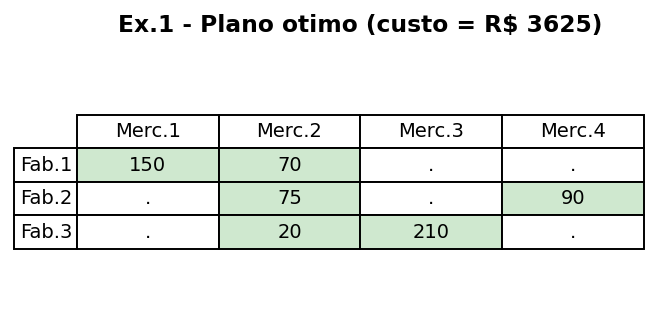
\includegraphics[width=0.78\linewidth]{p3_ex1_sol.png}
  \caption{Plano \'otimo de transporte, Parte 3, Exerc\'icio 1.}\end{figure}
\noindent\textbf{Custo m\'inimo} $=$ R\$ \textbf{3.625,00}, com
F1$\to$M1 (150), F1$\to$M2 (70), F2$\to$M2 (75), F2$\to$M4 (90),
F3$\to$M2 (20), F3$\to$M3 (210).

% ---------- Ex2 ----------
\subsection{Exerc\'icio 2: Compra de pneus (Expresso R\'apido Faxina)}
Modelado como transporte: ofertas = pneus dispon\'iveis por revendedor
$(A{=}12000,B{=}6000,C{=}4000)$; demandas = pneus necess\'arios por terminal
$(4000,8000,3000,5000)$. Oferta total $22000 > 20000$.
\begin{figure}[H]\centering
  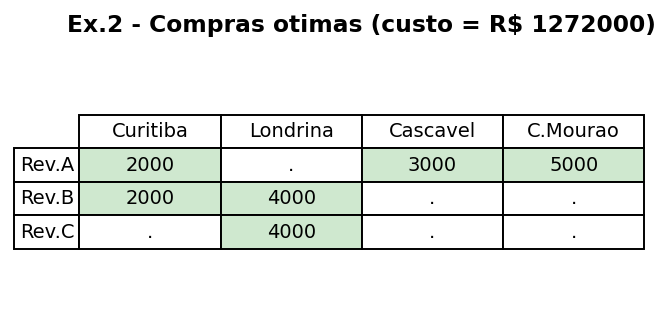
\includegraphics[width=0.82\linewidth]{p3_ex2_sol.png}
  \caption{Compras \'otimas (unidades por revendedor/terminal), Ex.\ 2.}\end{figure}
\noindent\textbf{Custo m\'inimo} $=$ R\$ \textbf{1.272.000,00}. Compra: do
Revendedor A $\to$ Cascavel (3000) e Campo Mour\~ao (5000) e parte de Curitiba
(2000); Revendedor B $\to$ Curitiba (2000) e Londrina (4000); Revendedor C $\to$
Londrina (4000). (Revendedor A fica com 2000 pneus de folga.)

% ---------- Ex3 ----------
\subsection{Exerc\'icio 3: Aquisi\c{c}\~ao de combust\'ivel}
Ofertas (mil gal\~oes) $(320,270,150)$; demandas $(100,180,300)$.
\begin{figure}[H]\centering
  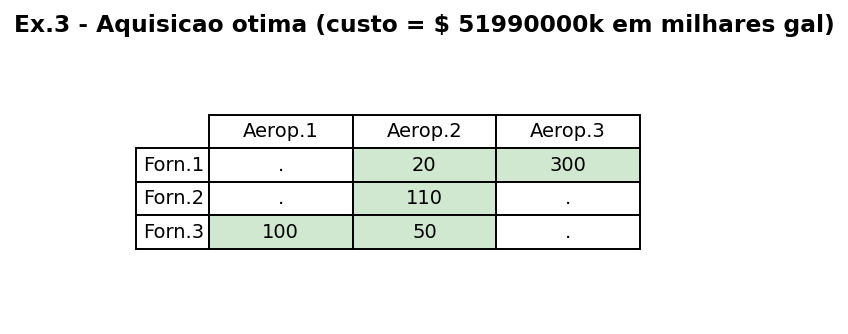
\includegraphics[width=0.7\linewidth]{p3_ex3_sol.png}
  \caption{Pol\'itica \'otima de aquisi\c{c}\~ao (mil gal\~oes), Ex.\ 3.}\end{figure}
\noindent\textbf{Custo m\'inimo} $=\$\,51.990$ (em mil gal\~oes $\times$ \$/gal\~ao),
isto \'e, \textbf{US\$ 51.990.000}. Pol\'itica: Forn.1 $\to$ Aerop.2 (20) e Aerop.3
(300); Forn.2 $\to$ Aerop.2 (110); Forn.3 $\to$ Aerop.1 (100) e Aerop.2 (50).

% ---------- Ex4 ----------
\subsection{Exerc\'icio 4: Mercados ``Deise-Luzia''}
Tr\^es centros $C_1,C_2,C_3$ (capacidades $500,750,400$) atendem 11 armaz\'ens
(demandas $112,85,138,146,77,89,101,215,53,49,153$). O custo \'e
$c_{ij}=0{,}50\cdot d_{ij}$ (\$/ton, onde $d_{ij}$ \'e a dist\^ancia em km da tabela).
\begin{figure}[H]\centering
  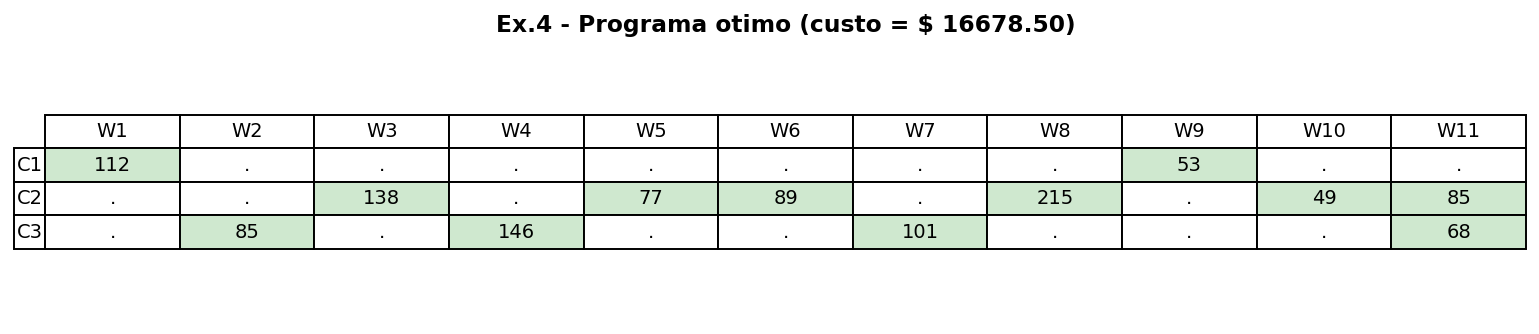
\includegraphics[width=\linewidth]{p3_ex4_sol.png}
  \caption{Programa \'otimo de transporte (toneladas), Ex.\ 4.}\end{figure}
\noindent\textbf{Custo m\'inimo} $=\$\,\textbf{16.678,50}$.

% ---------- Ex5 ----------
% \subsection{Exerc\'icio 5: Designa\c{c}\~ao (6 trabalhadores $\times$ 6 tarefas)}
% \begin{figure}[H]\centering
%   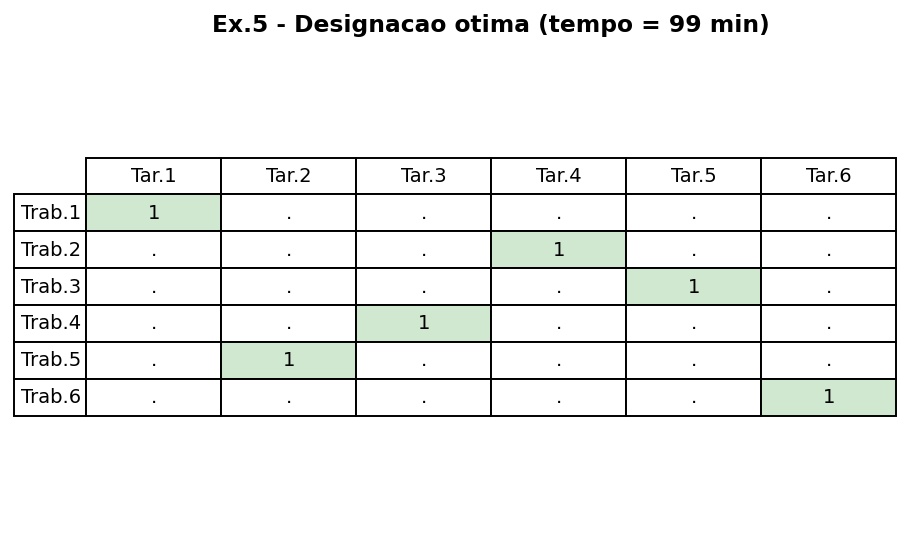
\includegraphics[width=0.72\linewidth]{p3_ex5_sol.png}
%   \caption{Designa\c{c}\~ao \'otima, Ex.\ 5.}\end{figure}
% \noindent\textbf{Tempo total m\'inimo} $=\textbf{99}$ minutos:
% T1$\to$Tarefa 1 (13), T2$\to$Tarefa 4 (18), T3$\to$Tarefa 5 (17),
% T4$\to$Tarefa 3 (13), T5$\to$Tarefa 2 (14), T6$\to$Tarefa 6 (24).

\newpage
% ============================================================================
\section{Parte 4: M\'inima Arboresc\^encia e Fluxo M\'aximo}
% ============================================================================
Para os problemas de grafos, foi utilizado a bibioteca \texttt{networkx} do Python para visualização do grafo.
\textbf{Observa\c{c}\~ao.} Os pesos/capacidades foram transcritos das figuras do
enunciado e reproduzidos nos grafos a seguir (para confer\^encia). Os algoritmos
foram implementados em Python.

% ---------- Ex1 ----------
\subsection{Exerc\'icio 1: M\'inima \'arvore geradora (Prim e Kruskal)}
\begin{figure}[H]\centering
  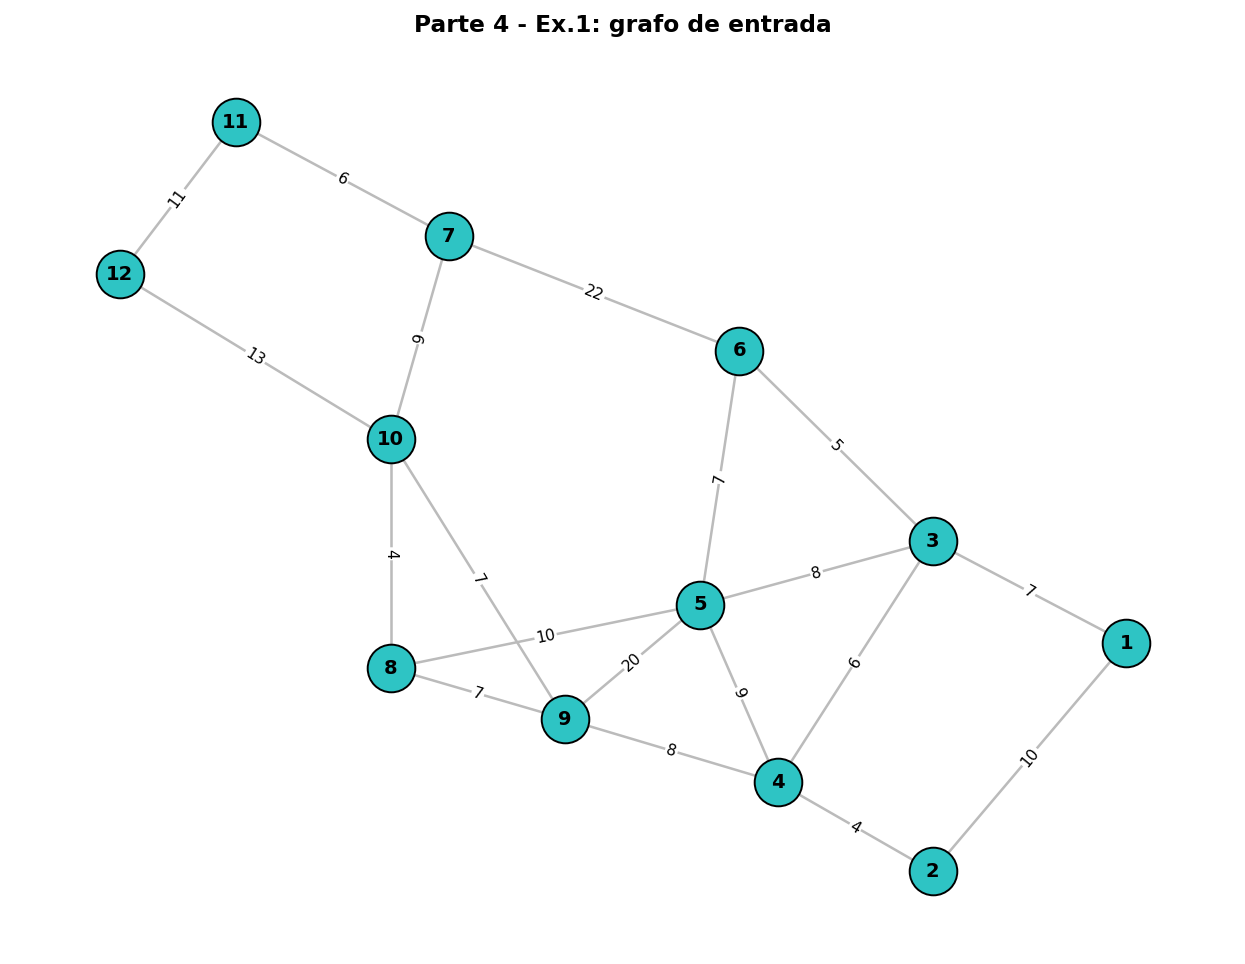
\includegraphics[width=0.62\linewidth]{p4_ex1_grafo.png}\hfill
  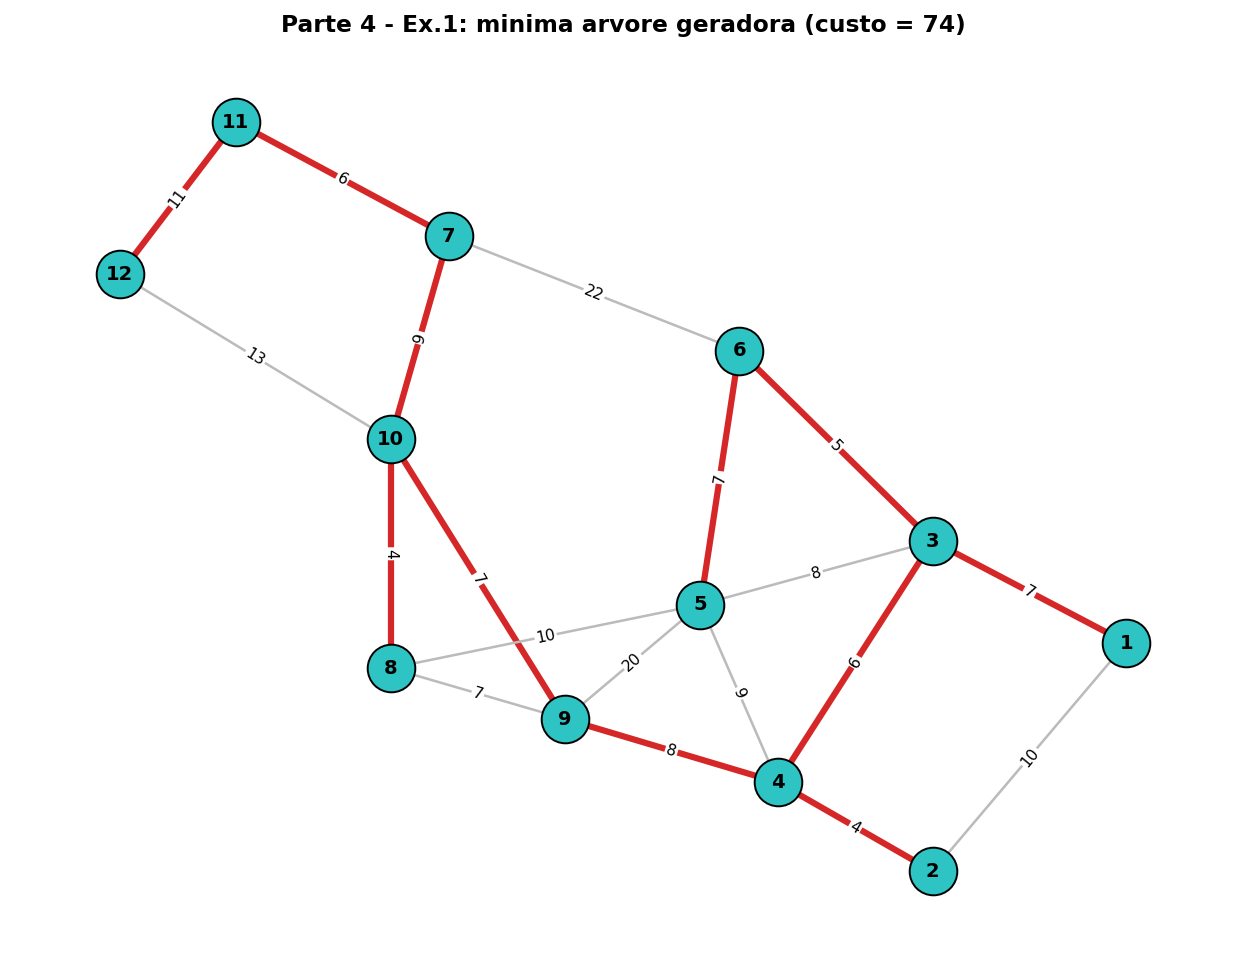
\includegraphics[width=0.62\linewidth]{p4_ex1_mst.png}
  \caption{Grafo de entrada (esq.) e \'arvore geradora m\'inima em vermelho
  (dir.), Ex.\ 1. Custo total $=74$.}\end{figure}

\noindent\textbf{Kruskal} (arestas em ordem n\~ao-decrescente de peso):
\begin{footnotesize}
\begin{longtable}{c c c c p{5.5cm}}
\toprule
Ordem & Aresta & Peso & Decis\~ao & Coment\'ario \\
\midrule
\endhead
1 & (10,8) & 4 & \textbf{aceita} & une componentes {10} e {8} \\
2 & (4,2) & 4 & \textbf{aceita} & une componentes {4} e {2} \\
3 & (6,3) & 5 & \textbf{aceita} & une componentes {6} e {3} \\
4 & (11,7) & 6 & \textbf{aceita} & une componentes {11} e {7} \\
5 & (3,4) & 6 & \textbf{aceita} & une componentes {3} e {4} \\
6 & (6,5) & 7 & \textbf{aceita} & une componentes {6} e {5} \\
7 & (3,1) & 7 & \textbf{aceita} & une componentes {3} e {1} \\
8 & (10,9) & 7 & \textbf{aceita} & une componentes {10} e {9} \\
9 & (8,9) & 7 & rejeita & formaria ciclo \\
10 & (3,5) & 8 & rejeita & formaria ciclo \\
11 & (9,4) & 8 & \textbf{aceita} & une componentes {9} e {4} \\
12 & (7,10) & 9 & \textbf{aceita} & une componentes {7} e {10} \\
13 & (5,4) & 9 & rejeita & formaria ciclo \\
14 & (8,5) & 10 & rejeita & formaria ciclo \\
15 & (1,2) & 10 & rejeita & formaria ciclo \\
16 & (11,12) & 11 & \textbf{aceita} & une componentes {11} e {12} \\
17 & (12,10) & 13 & rejeita & formaria ciclo \\
18 & (5,9) & 20 & rejeita & formaria ciclo \\
19 & (7,6) & 22 & rejeita & formaria ciclo \\
\bottomrule
\end{longtable}
\end{footnotesize}


% ---------- Ex2 ----------
\subsection{Exerc\'icio 2: M\'inima \'arvore geradora (Prim e Kruskal)}
\begin{figure}[H]\centering
  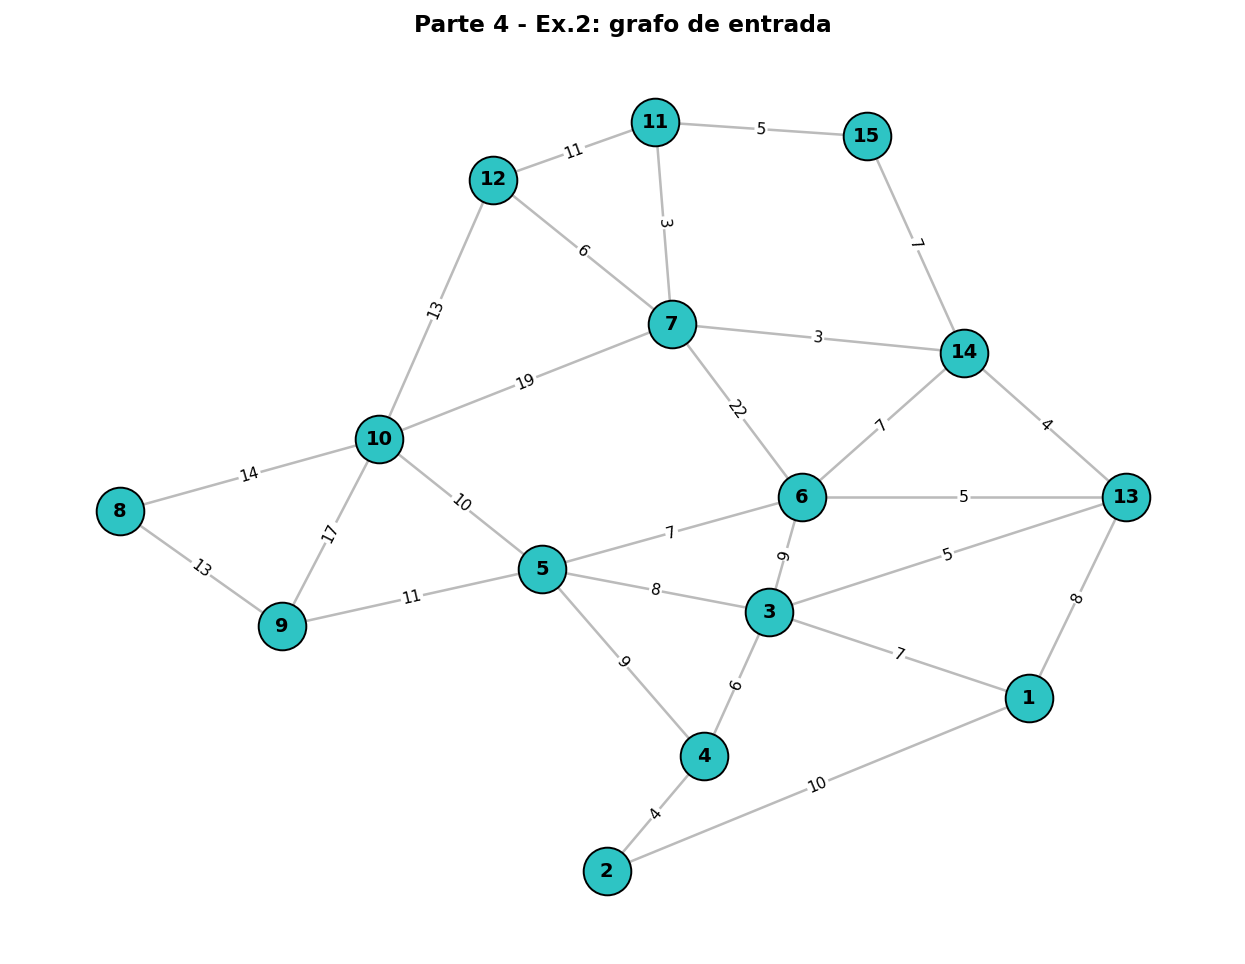
\includegraphics[width=0.62\linewidth]{p4_ex2_grafo.png}\hfill
  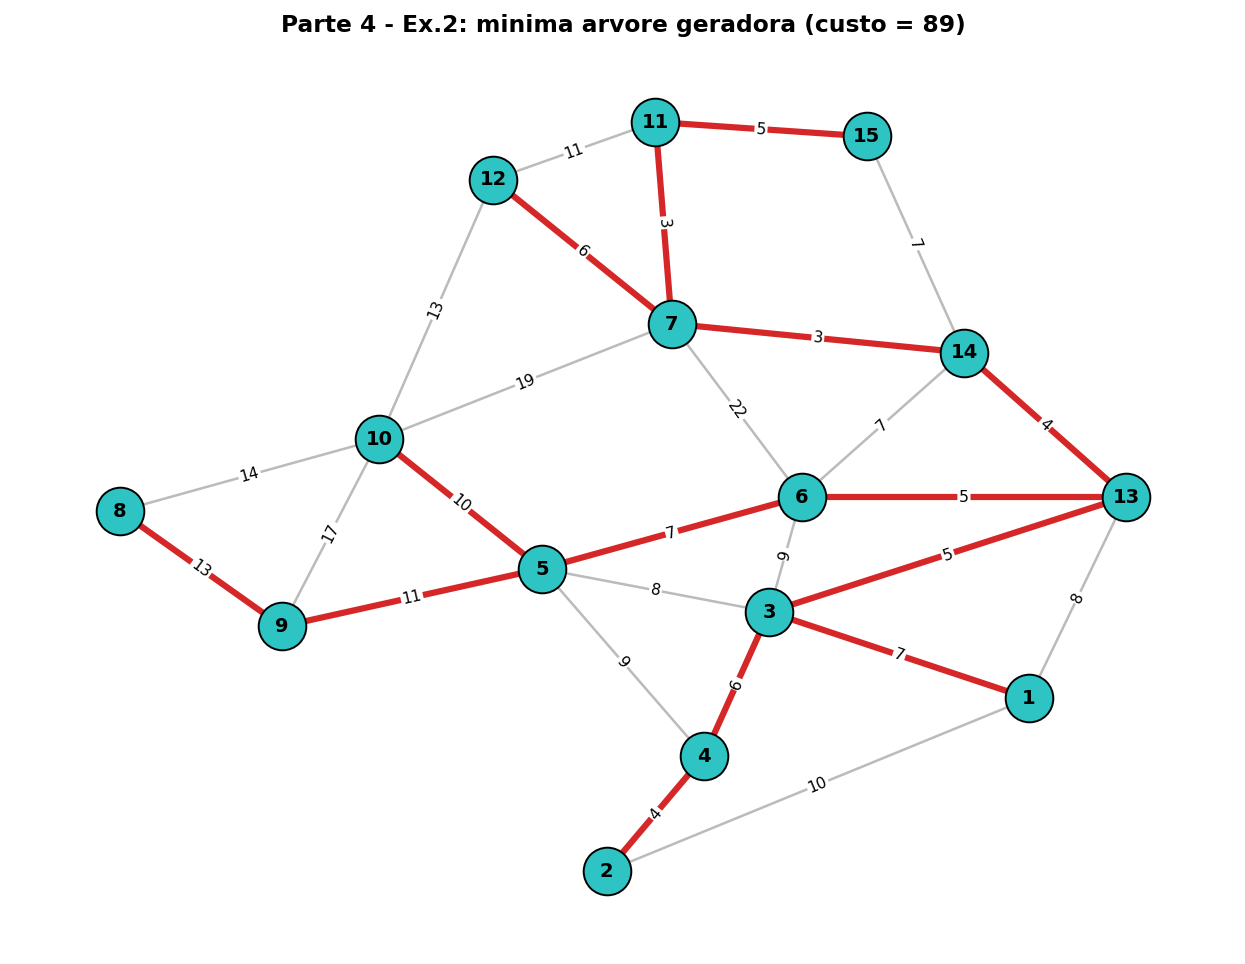
\includegraphics[width=0.62\linewidth]{p4_ex2_mst.png}
  \caption{Grafo de entrada (esq.) e \'arvore geradora m\'inima (dir.), Ex.\ 2.
  Custo total $=89$.}\end{figure}
\noindent\textbf{Prim} (a partir do n\'o 1):
\begin{footnotesize}
\begin{longtable}{c c c c p{5.5cm}}
\toprule
Itera\c{c}\~ao & Aresta & Peso & Decis\~ao & Coment\'ario \\
\midrule
\endhead
1 & (1,3) & 7 & \textbf{aceita} & adiciona no 3 via aresta (1,3) \\
2 & (3,13) & 5 & \textbf{aceita} & adiciona no 13 via aresta (3,13) \\
3 & (13,14) & 4 & \textbf{aceita} & adiciona no 14 via aresta (13,14) \\
4 & (14,7) & 3 & \textbf{aceita} & adiciona no 7 via aresta (14,7) \\
5 & (7,11) & 3 & \textbf{aceita} & adiciona no 11 via aresta (7,11) \\
6 & (11,15) & 5 & \textbf{aceita} & adiciona no 15 via aresta (11,15) \\
7 & (13,6) & 5 & \textbf{aceita} & adiciona no 6 via aresta (13,6) \\
8 & (3,4) & 6 & \textbf{aceita} & adiciona no 4 via aresta (3,4) \\
9 & (4,2) & 4 & \textbf{aceita} & adiciona no 2 via aresta (4,2) \\
10 & (7,12) & 6 & \textbf{aceita} & adiciona no 12 via aresta (7,12) \\
11 & (6,5) & 7 & \textbf{aceita} & adiciona no 5 via aresta (6,5) \\
12 & (5,10) & 10 & \textbf{aceita} & adiciona no 10 via aresta (5,10) \\
13 & (5,9) & 11 & \textbf{aceita} & adiciona no 9 via aresta (5,9) \\
14 & (9,8) & 13 & \textbf{aceita} & adiciona no 8 via aresta (9,8) \\
\bottomrule
\end{longtable}
\end{footnotesize}

\noindent Ambos os algoritmos produzem custo total $=\mathbf{89}$.

% ---------- Ex5 ----------
\subsection{Exerc\'icio 5: Fluxo m\'aximo (Edmonds-Karp)}
Grafo direcionado com 15 n\'os; fonte $s=1$, sumidouro $t=15$; capacidades dadas na
tabela do enunciado.

\textbf{Modelo matem\'atico} (fluxo m\'aximo). Seja $f_{ij}$ o fluxo no arco $(i,j)$
e $u_{ij}$ sua capacidade:
\[
\max\; F=\!\!\sum_{j:(1,j)\in A}\!\! f_{1j}
\qquad\text{s.a.}\qquad
\begin{cases}
\displaystyle\sum_{j:(i,j)\in A} f_{ij}-\!\!\sum_{j:(j,i)\in A} f_{ji}=0, & \forall i\neq 1,15\\[1ex]
0 \le f_{ij} \le u_{ij}, & \forall (i,j)\in A.
\end{cases}
\]
(conserva\c{c}\~ao de fluxo nos n\'os intermedi\'arios e limita\c{c}\~ao pela
capacidade dos arcos). O n\'ucleo do algoritmo de Edmonds-Karp (BFS no grafo
residual) \'e:
\begin{lstlisting}
from collections import deque
def edmonds_karp(nodes, arcs, s, t):
    cap = {}; adj = {v:set() for v in nodes}
    for u,v,c in arcs:
        cap[(u,v)] = cap.get((u,v),0)+c; cap.setdefault((v,u),0)
        adj[u].add(v); adj[v].add(u)
    flow = {k:0 for k in cap}; maxflow = 0
    while True:                                    # busca caminho aumentante
        prev = {s:None}; q = deque([s])
        while q:
            u = q.popleft()
            for v in adj[u]:
                if v not in prev and cap[(u,v)]-flow[(u,v)] > 0:
                    prev[v]=u; q.append(v)
        if t not in prev: break                    # nao ha mais caminho -> fim
        path=[]; v=t
        while prev[v] is not None: path.append((prev[v],v)); v=prev[v]
        b = min(cap[e]-flow[e] for e in path)      # gargalo
        for (u,v) in path: flow[(u,v)]+=b; flow[(v,u)]-=b
        maxflow += b
    return maxflow
\end{lstlisting}

\textbf{Passos do algoritmo} (caminhos aumentantes encontrados pela BFS e
respectivos gargalos):
\begin{footnotesize}
\begin{longtable}{c l c c}
\toprule
Itera\c{c}\~ao & Caminho aumentante (BFS) & Gargalo & Fluxo acumulado \\
\midrule
\endhead
1 & $1 \to  9 \to  3 \to  4 \to  15$ & 40 & 40 \\
2 & $1 \to  2 \to  3 \to  4 \to  15$ & 4 & 44 \\
3 & $1 \to  2 \to  3 \to  7 \to  15$ & 9 & 53 \\
4 & $1 \to  10 \to  3 \to  7 \to  15$ & 19 & 72 \\
5 & $1 \to  10 \to  6 \to  7 \to  15$ & 6 & 78 \\
6 & $1 \to  10 \to  6 \to  8 \to  15$ & 38 & 116 \\
7 & $1 \to  10 \to  6 \to  11 \to  15$ & 16 & 132 \\
8 & $1 \to  10 \to  14 \to  8 \to  15$ & 13 & 145 \\
9 & $1 \to  5 \to  3 \to  8 \to  15$ & 12 & 157 \\
10 & $1 \to  5 \to  3 \to  11 \to  15$ & 34 & 191 \\
\bottomrule
\end{longtable}
\end{footnotesize}


\noindent\textbf{Fluxo m\'aximo} $=\mathbf{191}$. Esse valor coincide com a soma das
capacidades dos arcos que saem da fonte ($13+46+40+92=191$): logo o
\emph{corte m\'inimo} \'e $(\{1\},\{2,\dots,15\})$ e todos os arcos da fonte
ficam saturados.
\begin{figure}[H]\centering
  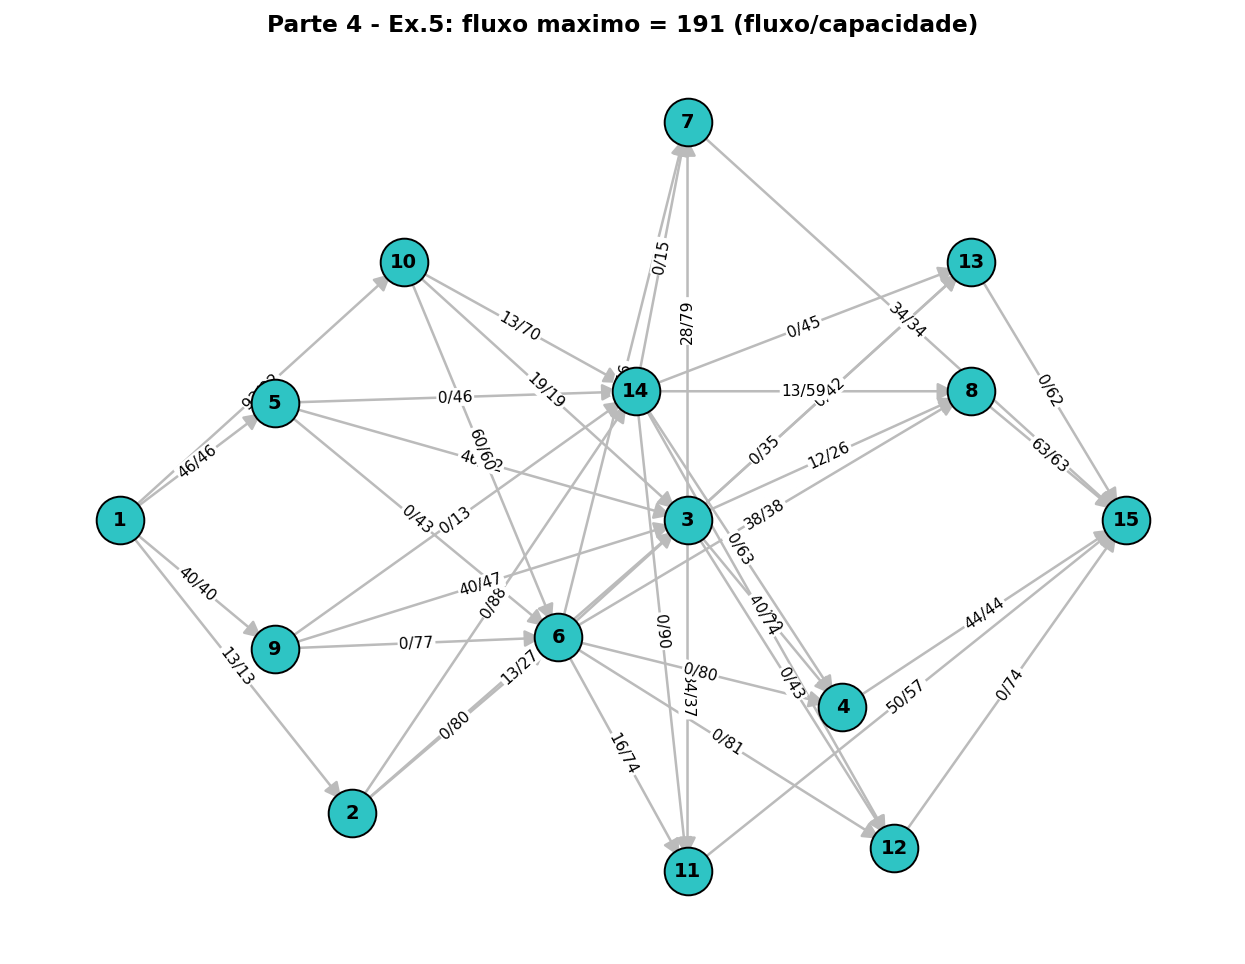
\includegraphics[width=0.92\linewidth]{p4_ex5_fluxo.png}
  \caption{Fluxo \'otimo (r\'otulos \emph{fluxo/capacidade}) --- Ex.\ 5.}\end{figure}

\end{document}
